%=========================
% Materials and Methods
%=========================


This research mainly examines relationships between the injuries caused by pests and diseases, production situations (e.g., rice varieties, crop establishments, fertilizer inputs, chemical applications), and rice yields using the data from surveys in irrigated lowland rice growing areas in South and South East Asia. I will develop and apply suitable methods of network analysis to characterize the patterns of co-occurrence of injuries and production situations. The resulting network of associations of injuries and production situations thus provides a starting point for further investigations of their relationships (i.e., comparison of networks from different production environments or examination of consequences of networks after imputation).

I propose three parts of network analysis of rice crop health survey. In the following, I present three distinct network analysis approaches: single-network analysis, differential network analysis, and dynamic network analysis. The three approaches answer different questions. 

In the first part of network analysis, I will apply single-network analysis in order to defines modules that can then be tested for validity with other data sets. Single-network analysis aims at identifying (a) patterns of interactions (modules) and (b) their key components (e.g., most connected variables) that are present in the data set.

The second part, differential network analysis, aims to uncover differences in the modules and connectivity between different data sets (e.g., dry season versus wet season). Each data set is then used to construct a network. Next, the networks are contrasted to find (1) non-preserved modules, (2) differentially occurred variables, and (3) differentially connected variables. 

Dynamic network analysis, in third part, is applied for study changes of networks at least two different aspects of an evolving complex system. Here I vary yield, and obtain different yield data set in order to construct a dynamic network of yield varying behaviors.  Similar to differential network analysis, dynamic network focus on comparison of network structure, but it enable us to observe networks changing across successive yield gains. 


\subsection*{Crop Health Survey Data}
% which crop health survey data? The data used in this research? Also, why several seasons? Get to the point. Which years and seasons?

% not necessary to say "at all fields" you already said "using the same protocol".
The crop health survey data were generated from surveys of farmers' fields in several seasons and production environments across South and South East Asia, specially in irrigated lowland rice growing areas (West Java, Indonesia; Mekong River Delta and Red River Delta, Vietnam; Tamil Nadu and Odisha, India; and Suphanburi, Thailand) from 2009 to 2015. They were conducted using the same protocol \cite{Savary:1996ud}. 

The survey data consist of measures of multiple variables with different types of value. Data were divided each sample into three sets of variables, production situation set, injuries and disease set, and yield. \textbf{cropping practice set} are simplified, which collected with many type of data. For example, type of rice varieties (traditional varieties, modern varieties, and hybrid rice), crop establishments ( direct seeded, transplanted rice) were collected in categorical data, pesticide (molluscicide, herbicide, insecticide and fungicide) uses were collected discretized data, and accumulated organic, chemical fertilizers were collected in continuous data. \textbf{Injuries and diseases set} composted of specific signs caused by pests or pathogens (i.e., whitehead, brown spot). They are collected percent of incidence of injury at two rice stages.Two types of injury indices were used areas under progress curves or maximum level of injuries or disease incidence depending on the nature of the injury. The time-dependent information on injuries was thus synthesized and compacted over time.

Samples composed of incomplete data were removed. These were encoded as a matrix in which each row represented a surveyed field in a specific location, year and season. Each column represented a collected variables.


\section*{Single Network Development}


In the case of single network analysis, one use single network for modeling the relationship of cropping practice set, and injuries and disease sets. In the following, I describe a typical single-network analysis for finding the patterns of relationships.
While a single network is the focus, it does not imply that only a single data set is used. Instead, appropriately similar multiple data sets can be used to validate the robustness of module definition and connectivity.

In the following, we provide an overview of single- network analysis strategy, which is depicted in Fig. 1: (a) process data preparation. (b) Calculate correlation coefficients (Pearson, Spearman, or Kendall). Estimate P-values for all coefficients. Next, determine threshold values for the resulting correlation coefficients and \textit{P} values, storing results in adjacency matrices for the construction of networks. (c) Construct network and analyze network for graph-theoretic properties and infer biological meanings and integrate the network of input data and output data. (d) yield- related variables are used to prioritize variables within crop health data

\subsection*{Evaluation of pairwise relationship association methods for network construction}

This research aims to construct networks visualizing the associations of injuries from pests and diseases with production situations. The rules defining edges of such networks is to present a sufficient level of 'association' between certain attributes of the two nodes. I thus choose correlation measurements to construct an association network based on them.

% Don't forget punctuation. You left a "." off the last sentence.
%A correlation matrix describes pairwise associations between variables and therefore can be used for estimating such a network structure. I can compute Pearson correlations on this dataset. There are several techniques to determine the correlation between variables; mainly using either Pearson's or Spearman's correlations for data \shortcite{qin2010human, Barberan:2012bd}.

To identify the most appropriate method for constructing a network based on correlation measurements, I select four correlation based measures, Pearson's correlation, Spearman's rank correlation, Kendall's correlation, Biweight midcorrealtion. The cor.test function of R \shortcite{rprogram} is applied for generating a correlation matrix, which describes the pairwise associations between variable in the context of the crop health survey data. This function allow users to select type of correlation measures to perform such as Pearson's correlation, Spearman's rank correlation and Kandell's rank correlation. "bicor" function of WGCNA package \shortcite{Langfelder:2008bd} in R is applied for computing biweight midcorrelation matrix. A corresponding correlation matrix describes pairwise associations between variables is create. % I'm really not sure what's going on here?

When correlation matrix was create, next is to remove spurious relationships or rank-based correlation coefficients, which are applied on the investigated data profiles. Removal of spurious relationships is of particular importance when one attempts to establish causal relations between variables.

%Constructing the [weighted (Box 1d)] network from the similarity matrix requires the application of a statistically sound threshold, which can be principally obtained in two ways: (i) Determine P values for all similarities (followed in [60,61]) and adjust them for multiple hypotheses testing (e.g., Bonferroni or local false- discovery rate [62]). Edges are then established only for entries of the similarity matrix that are statistically sig- nificant at a pre-specified level a (followed in [63]), often calculated with the aid of permutation tests. Motivated by the interest in the strongest relationships, one may further filter for entries in the similarity matrix above a fixedthreshold (e.g., as used in [56]). (ii) Obtain a threshold value that guarantees a pre-specified false-discovery rate. Edges are then established only for entries of the similarity matrix, which are above the obtained threshold [64].


% Here is on how to determine the best opt measures of correlation  matrix to the 


%Although we can opt for a method based on its principle of statistical operation without paying attention to the biological models in a given data set, this may not lead to a coordination network that will reveal biological knowledge. High dimensional biological data from microarray or high throughput sequencin data often contain at least a few hundred different biological processes. There is no statistical method that is suitable for all of them. Identification of the most efficient method for knowledge discovery of a specific biological process demands concrete prediagnostic analyses. Based on our study and our empirical knowledge, we would suggest the following procedure for identifying the most appropriate gene association method for a specific biological theme in a given data set: (1) Evaluate the prior knowledge of biological processes of one’s interest, and select a few known genes involved in these processes; (2) Use the R codes from this study to perform a genome-wide coexpression analysis to obtain the top 100 or 500 genes that are most closely associated to the selected known genes; (3) Perform an evaluation of these 100 or 500 genes by examining which methods can associate the more functionally relevant genes to the selected genes. This can be achieved by examining gene annotation or performing GO term enrichment analysis: and (4) Choose the best method for the data. However, if prior knowledge of biological theme of one’s interest is lacking, we suggest the most stable gene association method. 

% I don't agree with your first sentence. The network won't reveal knowledge. Knowledge comes with understanding. 
% Sloppy spelling in this para.

%Although we can opt for a method based on its principle of statistical operation without paying attention to the biological models in a given data set, this may not lead to a coordination network that will reveal biological knowledge. High dimensional biological data from microarray or high throughput sequencin data often contain at least a few hundred different biological processes. There is no statistical method that is suitable for all of them. Identification of the most efficient method for knowledge discovery of a specific biological process demands concrete pre- diagnostic analyses. Based on our study and our empirical knowledge, we would suggest the following procedure for identifying the most appropriate gene association method for a specific biological theme in a given data set: (1) Evaluate the prior knowledge of biological processes of one’s interest, and select a few known genes involved in these processes; (2) Use the R codes from this study to perform a genome-wide coexpression analysis to obtain the top 100 or 500 genes that are most closely associated to the selected known genes; (3) Perform an evaluation of these 100 or 500 genes by examining which methods can associate the more functionally relevant genes to the selected genes. This can be achieved by examining gene annotation or performing GO term enrichment analysis: and (4) Choose the best method for the data. However, if prior knowledge of biological theme of one’s interest is lacking, we suggest the most stable gene association method. 


%The resulting network of  associations thus provides a starting point for further investigations of the ecological mechanisms underlying the establishment and maintenance of human microbiome structure.
% This is unclear "This part is composed of network structure characterization, module detection, the associations of network properties to environment characteristics." the last part needs clarification starting with "the associations"
% edits for clarity

% You propose to apply network analysis to survey DATA


\section*{Differential Network Analysis} 

%The second part is network analysis. This part is composed of network structure characterization, module detection, the associations of network properties to environment characteristics. 

%Finally, the network differences can be compared under different conditions and locations to analyze the effect of environments on network structure and interactions.

%For this research, I will construct networks from different sets of data (e.g., from different locations and years), structural properties can be used to determine the differences between the networks \cite{Subramanian2005}. Differential networks are illustrated in Figure \ref{fig:wholenet}.

% So the components are contributing to rice yield losses in a systematic perspective?
Networks allow one to look at components contributing to rice yield losses in systematic perspective. For instance, how are whitehead injuries related to type of crop establishment, or might leaf blast be related to insect pest injuries, or if a farmer used a direct seeding method, how are the risk of insect pests and other yield reducing factors related to this crop establishment method. This type of understanding is important, because if we can predict the key pests, then it is possible recommend a suitable pest management strategy for a given situation. It is anticipated that interesting connections between the individual inputs defined in production situation and single variable of injury profiles might appear through a network that have yet to be seen by more conventional approaches. I propose to collect the two types of profiling data; one is input profiling data, and another is output profiling data.  The construction of networks from crop health survey data are illustrated in Figure \ref{fig:pipeline}.

% why is 2.3 not 2.1? % The problem there is that you must put the label after a caption, so the label can reference to the figure (it references to the caption, actually). See here: http://www.latex-community.org/forum/viewtopic.php?t=3659 I've corrected this. - ahs
 
%We describe another application of WGCNA, differential network analysis, which may be useful in identifying gene pathways distinguishing phenotypically distinct groups of samples. In our example, we identified the 30 mice at both extremes of the weight spectrum in the B · H data and constructed the first network using the 30 leanest mice and the second network using the 30 heaviest mice. For the ith gene, we denote by k1(i) and k2(i) the whole-network connectivity in networks 1 and 2, respectively. To facilitate the comparison between the connectivity measures of each network, we divide each gene connectivity by the maxi- mum network connectivity, i.e.,

\section*{Dynamic Network Analysis}

% not yet finished


\subsection*{Analyzing the Structure of Network Models}

% edited for Tex code
Once networks are constructed, several indices can be computed that convey information about network structure. Structural properties of networks can be used for the interpretation of datasets and for generating hypotheses. Two types of structure are important. First, typically one is interested in the global structure of the network (random networks, small networks, scale-free networks) \shortcite{Strogatz:2001wc, Jeger:2007tn}. Second, one may be interested in local patterns, which are characteristics of each node. For example, clustering of nodes and/or edges in a network can identify groups of nodes with similar properties, and these are referred to ``modules'' or ``communities''  \shortcite{osorio2012integrative, Jeger:2007tn}.

% edited for clarity
For deep insights, comparing the networks by using some key topological properties of network are usefully conducted. Degree and degree distribution of a network is a simple property to extract from network models, which are the number of connections of each node and the frequency distribution of the number of connections per node, respectively. Cluster coefficient is the other measure, which is the value that is able to indicate whether the entities in network form cluster or group within network structure. \shortciteA{Deng:2012do, newman2003structure, Toubiana:2013cv} are recommended references for descriptions of the network properties as well as the formal calculation of these measures.


\begin{landscape}

\begin{figure}[h!]
\centering
%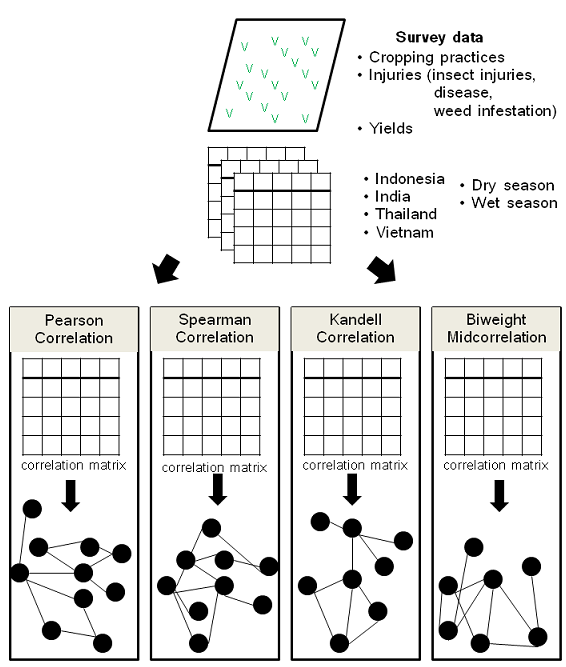
\includegraphics[resolution = 600]{pipeline}
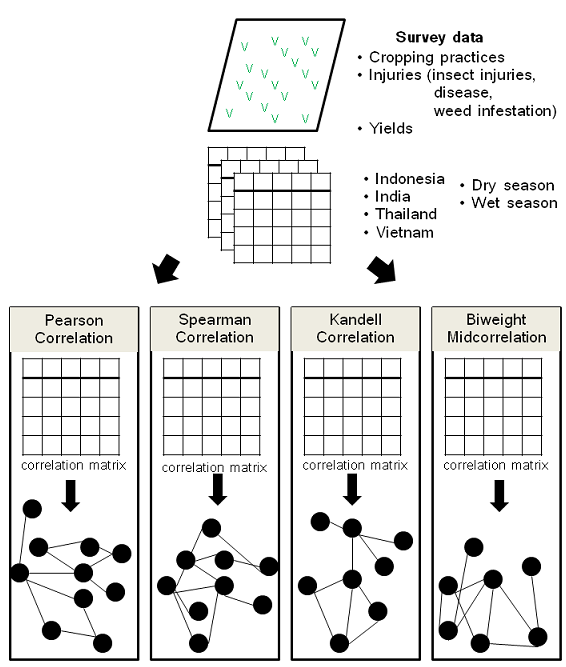
\includegraphics[width=6in]{pipeline}

\caption[Proposed pipeline for network construction]{Proposed pipeline for network construction. (a) Collect the input profiling data and output profiling data from different samples and different locations. (b) Calculate correlation coefficients (Pearson, Spearman, or Kendall). Estimate P-values for all coefficients. Next, determine threshold values for the resulting correlation coefficients and \textit{P} values, storing results in adjacency matrices for the construction of networks. (c) Construct network and analyze network for graph-theoretic properties and infer biological meanings and integrate the network of input data and output data. (d) Repeat analysis for a second season to verify the network model.}
\label{fig:pipeline}
\end{figure}
\end{landscape}

\newpage
\begin{landscape}
\begin{figure}[h!]
\centering
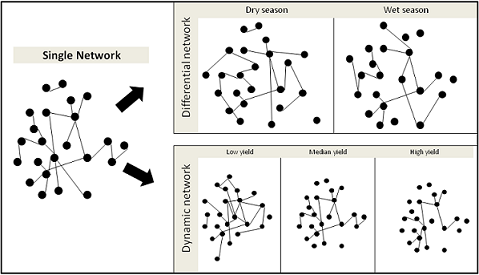
\includegraphics[width=6in]{wholenet}

\caption[Network comparison]{Network comparison: Network models constructed from survey datasets of different geographic locations are compared by determining their properties. Networks will express the conserved domains within their structure. A merged representation of the two networks being compared is also proposed as a holistic network of rice ecosystem in South and South East Asia.}
\label{fig:wholenet}
\end{figure}
\end{landscape}


